As mentioned above, this project starts with data collection. Since data is the basis of this project, it is worth spending more time on data collection and preprocessing. Once the data is processed, re-implementation and algorithm design will be commenced. Ideal due of those stages is before the end of autumn semester (or before the start of spring semester). In the spring semester, the focus will be experiment, evaluation, improvement and writing paper. Such arrangement ensures that the whole project runs in steady at an early stage and reserves enough time for handling contingency. The Gantt chart following shows the preliminary schedule of this project, consisting tasks below (note that events such as exams are excluded in this schedule, some tasks will commence in parallel):
\begin{enumerate}
    \item Literature search (3 weeks)
    \item Complete project proposal (1-2 weeks)
    \item Data collection and preprocessing (5-7 weeks)
    \item Write interim report (7-8 weeks)
    \item Algorithm design and implementation (about 10-13 weeks)
    \item Write final dissertation (at most 16 weeks)
    \item Re-implement others’ work (about 6 weeks)
    \item Test and evaluate the performance of the algorithm and compare with previous work (2-3 weeks)
    \item Review the whole project and do final adjustment (5 weeks)
    \item Prepare for demonstration (2 weeks)
\end{enumerate}
	
\begin{figure}[htbp]
    \centering
    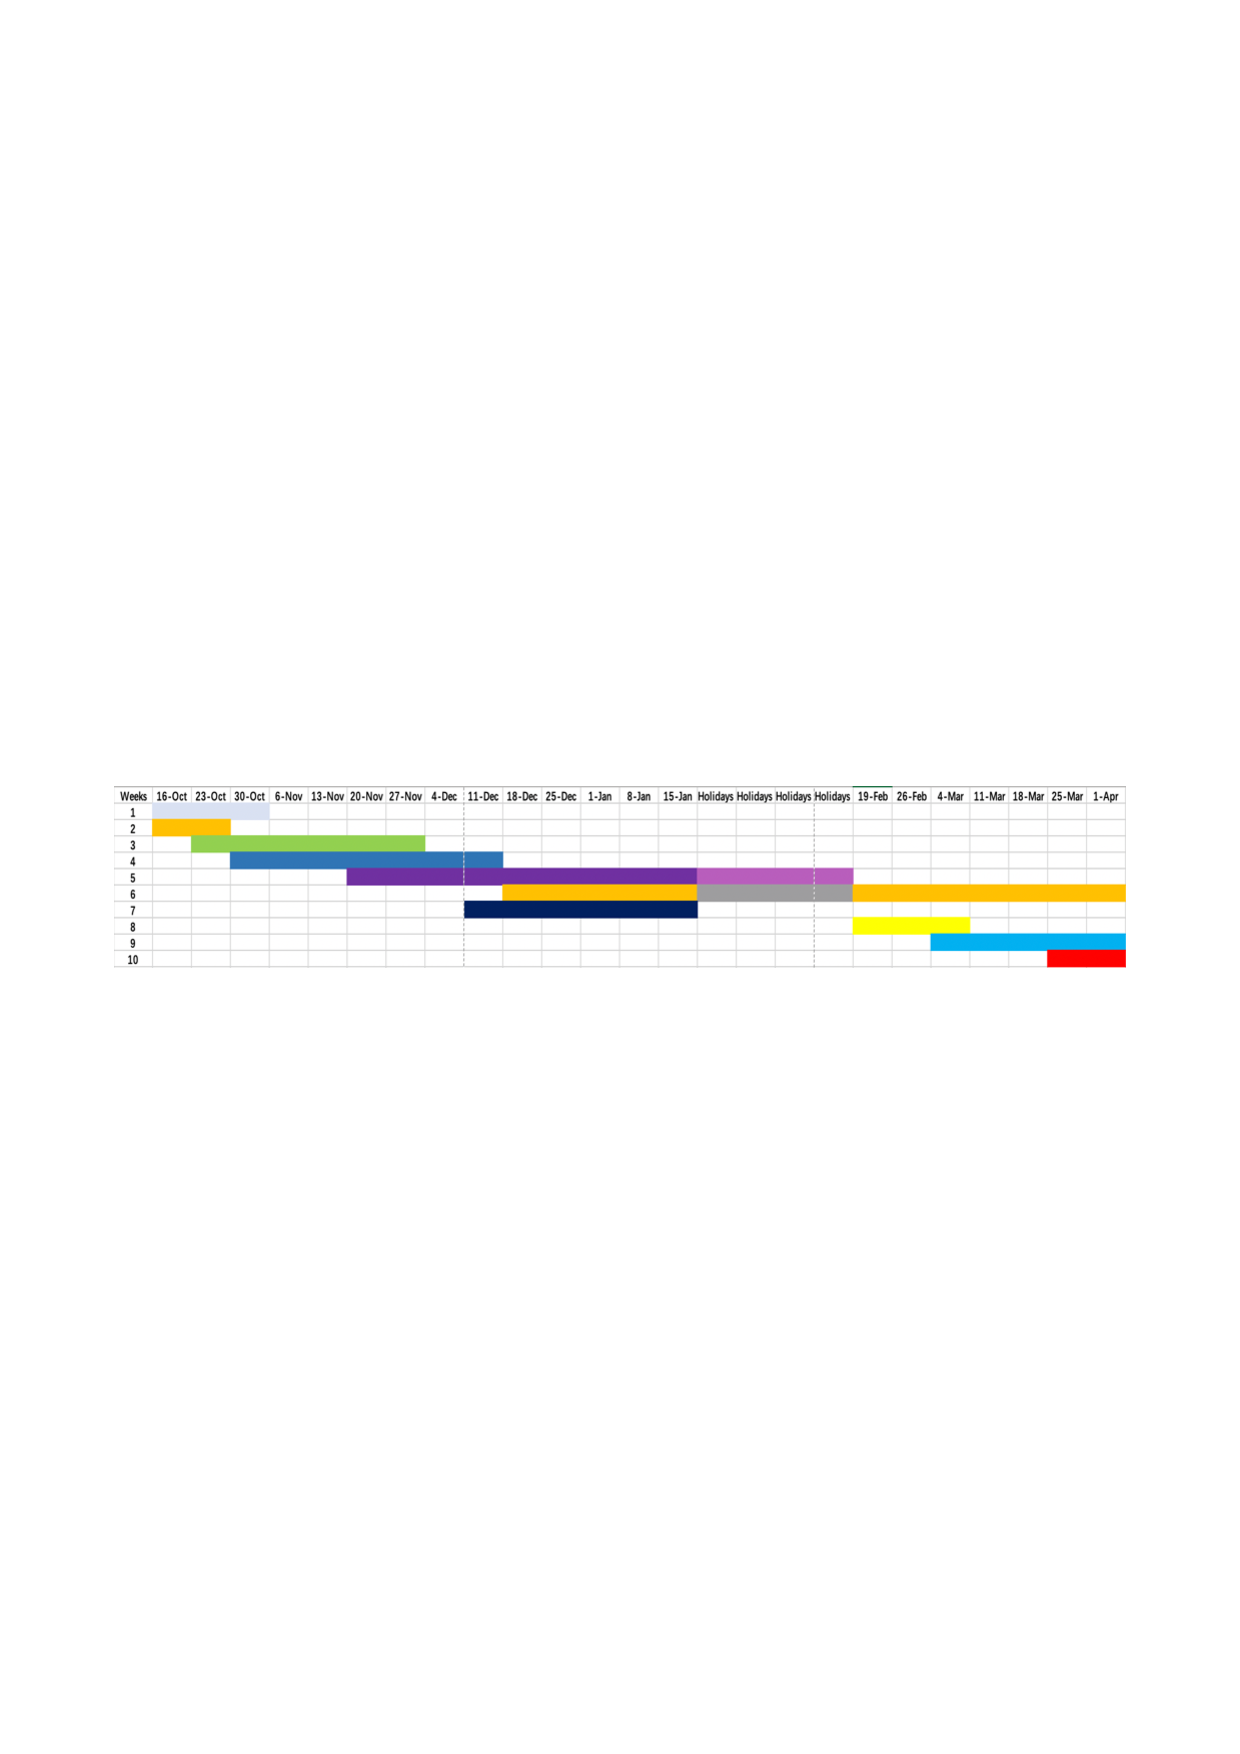
\includegraphics{pic1.pdf}
    \caption{Schedule}
    \label{fig1}
    \end{figure}
